\documentclass[12pt, a4paper]{article}
\usepackage[francais]{babel}
\usepackage{caption}
\usepackage{graphicx}
\usepackage[T1]{fontenc}
\usepackage{listings}
\usepackage{geometry}
\usepackage{minted}
\usepackage{array,multirow,makecell}
\usepackage{float}
\usepackage[colorlinks=true,linkcolor=black,anchorcolor=black,citecolor=black,filecolor=black,menucolor=black,runcolor=black,urlcolor=black]{hyperref}
\setcellgapes{1pt}
\makegapedcells
\usepackage{fancyhdr}
\pagestyle{fancy}
\lhead{}
\rhead{}
\chead{}
\rfoot{\thepage}
\lfoot{Baumgaertner - Rehm - Doghmane}
\cfoot{}
\renewcommand{\footrulewidth}{0.4pt}
\renewcommand{\headrulewidth}{0.4pt}
\renewcommand{\listingscaption}{Code}
\renewcommand{\listoflistingscaption}{Table des codes}

% \usepackage{mathpazo} --> Police à utiliser lors de rapports plus sérieux

\begin{document}
\begin{titlepage}
	\newcommand{\HRule}{\rule{\linewidth}{0.5mm}} 
	\center 
	\textsc{\LARGE iut de colmar}\\[4.5cm] 
	\textsc{\Large SAE 24}\\[0.5cm] 
	\textsc{\large projet intégratif}\\[0.5cm]
	\HRule\\[0.75cm]
	{\huge\bfseries Partie Web - Base de données}\\[0.4cm]
	\HRule\\[1.5cm]


	% Utiliser les lignes qui suivent dans le cas où il y a plusieurs membres
	%------------------------------------
	\begin{minipage}{0.4\textwidth}
		\begin{flushleft}
			\large
			\textit{RT11}\\
			Martin \textsc{Baumgaertner}
		\end{flushleft}
	\end{minipage}
	~
	\begin{minipage}{0.4\textwidth}
		\begin{flushright}
			\large
			\textit{RT12}\\
			Mehdi \textsc{Rehm}
		\end{flushright}
	\end{minipage}
    \\[0.7cm]
    \begin{minipage}{0.4\textwidth}
		\begin{flushleft}
			\large
			\textit{RT11}\\
			Sâji \textsc{Doghmane}
		\end{flushleft}
	\end{minipage}
	~
    \begin{minipage}{0.4\textwidth}
		\begin{flushright}
			\large
			\textit{\textcolor{white}{Mehdi}}\\
			\textcolor{white}{Mehdi} \textsc{\textcolor{white}{Mehdi}}
		\end{flushright}
	\end{minipage}
    
	%------------------------------------
    %------------------------------------
	% \textsc{\large martin baumgaertner}\\[0.5cm] % S'il y que moi qui écrit
    %------------------------------------
	\vfill\vfill\vfill
	{\large\today} 
	\vfill
\end{titlepage}
\newpage
\tableofcontents
\listoflistings
\listoffigures
\newpage



\newpage
\section{Introduction}
Le but de cette dernière partie est de pouvoir afficher sur une page web que nous
développons en Django les valeurs de températures avec plusieurs types de complications. 
Par exemple, nous devons être capable de lister les données de températures en fonction d'un
capteur, ou de proposer des modifications de champs. 

\section{Mise en place du projet Django}
\subsection{Connexion du projet Django à la base de données}
	Pour pouvoir connecter notre projet à la base de données que nous avions remplie
	dans la partie précédente avec le script de récupération des données, nous devons 
	modifier le fichier \texttt{settings.py} de notre projet Django.

	\begin{listing}[H]
		\caption{Configuration de \texttt{settings.py}}
		\label{lst:settings}
		\begin{minted}{py}
	DATABASES = {
		'default': {
			'ENGINE': 'django.db.backends.mysql',
			'NAME': 'temp', 
			'USER': 'martin',
			'HOST': '10.37.129.3',
			'PORT': '3306',
			'PASSWORD': 'martin',
		}
	}
		\end{minted}
	\end{listing}

	Nous mettons l'adresse \texttt{10.37.129.3}, qui correspond à l'adresse de ma machine 
	windows où est herbergée notre base de données. Puis, le nom de
	notre base de données est \texttt{temp}. Enfin, \texttt{martin} correspond au nom utilisateur
	avec le mot de passe \texttt{martin}. J'ai au préalable créé cet utilisateur et 
	autorisé la connexion depuis la machine où est mon projet Django.
	
	\newpage
	L'adresse IP \texttt{10.37.129.4} correspond à l'adresse de ma machine où je fais 
	mon projet Django. 
	Pour créer cet utlisateur, lui donner tous les droits et l'autoriser à se connecter il faut
	utiliser les commandes suivantes :
	\begin{listing}[H]
		\caption{Création de l'utilisateur}
		\label{lst:user}
		\begin{minted}{mysql}
	CREATE USER 'martin'@'10.37.129.4' IDENTIFIED BY 'martin';
	GRANT ALL PRIVILEGES ON *.* TO 'martin'@'10.37.129.4';
	FLUSH PRIVILEGES;
		\end{minted}
	\end{listing}

	\subsection{Récupération des tables}

	Nous pouvons donc désormais nous connecter à la base de données
	depuis le projet Django, et faire un \texttt{python3 manage.py makemigrations} 
	et \texttt{python3 manage.py migrate} pour que les données soient migréées. 
	Toutes les tables sont sauvegardées et nous observons que les tables que Django
	créee lors de la migrations du projet sont bien présentes :
	\begin{figure}[H]
		\centering
		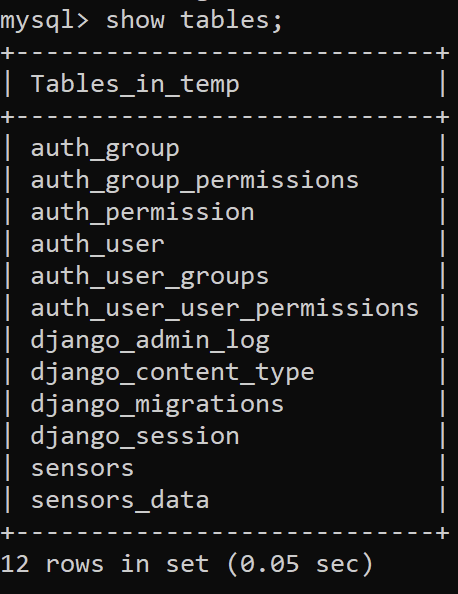
\includegraphics[width=0.4\textwidth]{../img/tables.png}
		\caption{Les tables créées par Django}
		\label{fig:tables}
	\end{figure}
	\newpage
	\section{Développement}
	\subsection{Création du fichier \texttt{models.py} à partir de la base de données}
	Ensuite, nous allons créer le fichier \texttt{models.py} qui va permettre de créer les modèles 
	nécessaire pour la suite du projet. Pour ce faire, nous allons utiliser la commande suivante :
	\begin{listing}[H]
		\caption{Création du fichier \texttt{models.py}}
		\label{lst:models}
		\begin{minted}{shell}
		python3 manage.py inspectdb > models.py 
		\end{minted}
	\end{listing}
	Suite à cela, notre fichier est bien créé et nous pouvons commencer le développement.\\[0.5cm]
	\subsection{Affichage des 2 capteurs sur une page d'accueil}
	Nous nous retrouvons donc avec les 2 capteurs, je veux les afficher sur une page d'accueil.
	Pour ensuite permettre à l'utilisateur de naviguer à travers les données des capteurs en 
	fonction du capteur qu'il sélectionne.
	Premièrement je fais une "vue all" pour récupérer les informations des deux capteurs :
	\begin{listing}[H]
		\caption{Création de la vue \texttt{all}}
		\label{lst:all}
		\begin{minted}{python}
def index(request): 
    sensors = Sensors.objects.all()
    sensorsdata = SensorsData.objects.all()
    return render(request, 'index.html', {'sensors': sensors})
		\end{minted}
	\end{listing}
	\newpage
	Avec un peu de développement HTML et CSS nous obtenons ce style de page, qui nous permet d'avoir
	les deux capteurs sur une seule page :\\
	\begin{figure}[H]
		\centering
		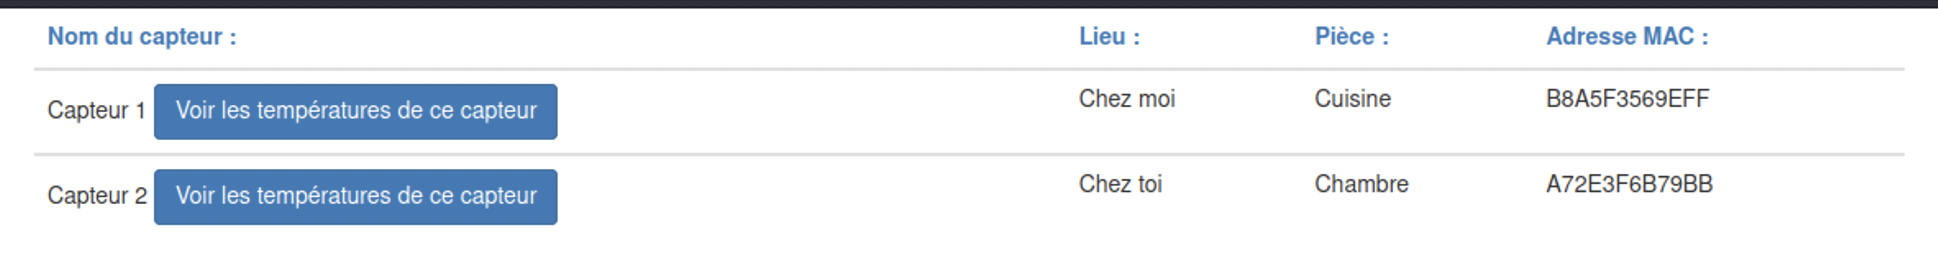
\includegraphics[width=1\textwidth]{../img/index.png}
		\caption{Page d'accueil}
		\label{fig:index}
	\end{figure}
	Avoir fait le choix d'avoir uniquement quelques éléments sur la page d'accueil, donc ici
	les 2 capteurs permet de ne pas surcharger la page d'index et d'avoir un rendu minimaliste
	que j'apprécie tout particulièrement.\\

	\subsection{Affichage des données en fonction d'un capteur}
	Pour pouvoir afficher les valeurs d'un capteur en fonction de celui que l'on choisit nous 
	mettre en place un filtre qui sélectionne les données du capteur que l'on veut afficher.
	Pour ce faire, je vais créer cette vue :
	\begin{listing}[H]
		\caption{View pour afficher les données d'un capteur}
		\label{lst:sensor}
		\begin{minted}{python}
def temp(request, id):
	temp = SensorsData.objects.filter(sensor__id=id)
	return render(request, 'data.html', {'temp': temp})
		\end{minted}
	\end{listing}

	\newpage

	Encore une fois, avec un peu de HTML et de CSS, nous arrivons assez facilement à générer ce 
	genre de tableau pour lister les données du capteur de température choisi :\\[1cm]
	\begin{figure}[H]
		\centering
		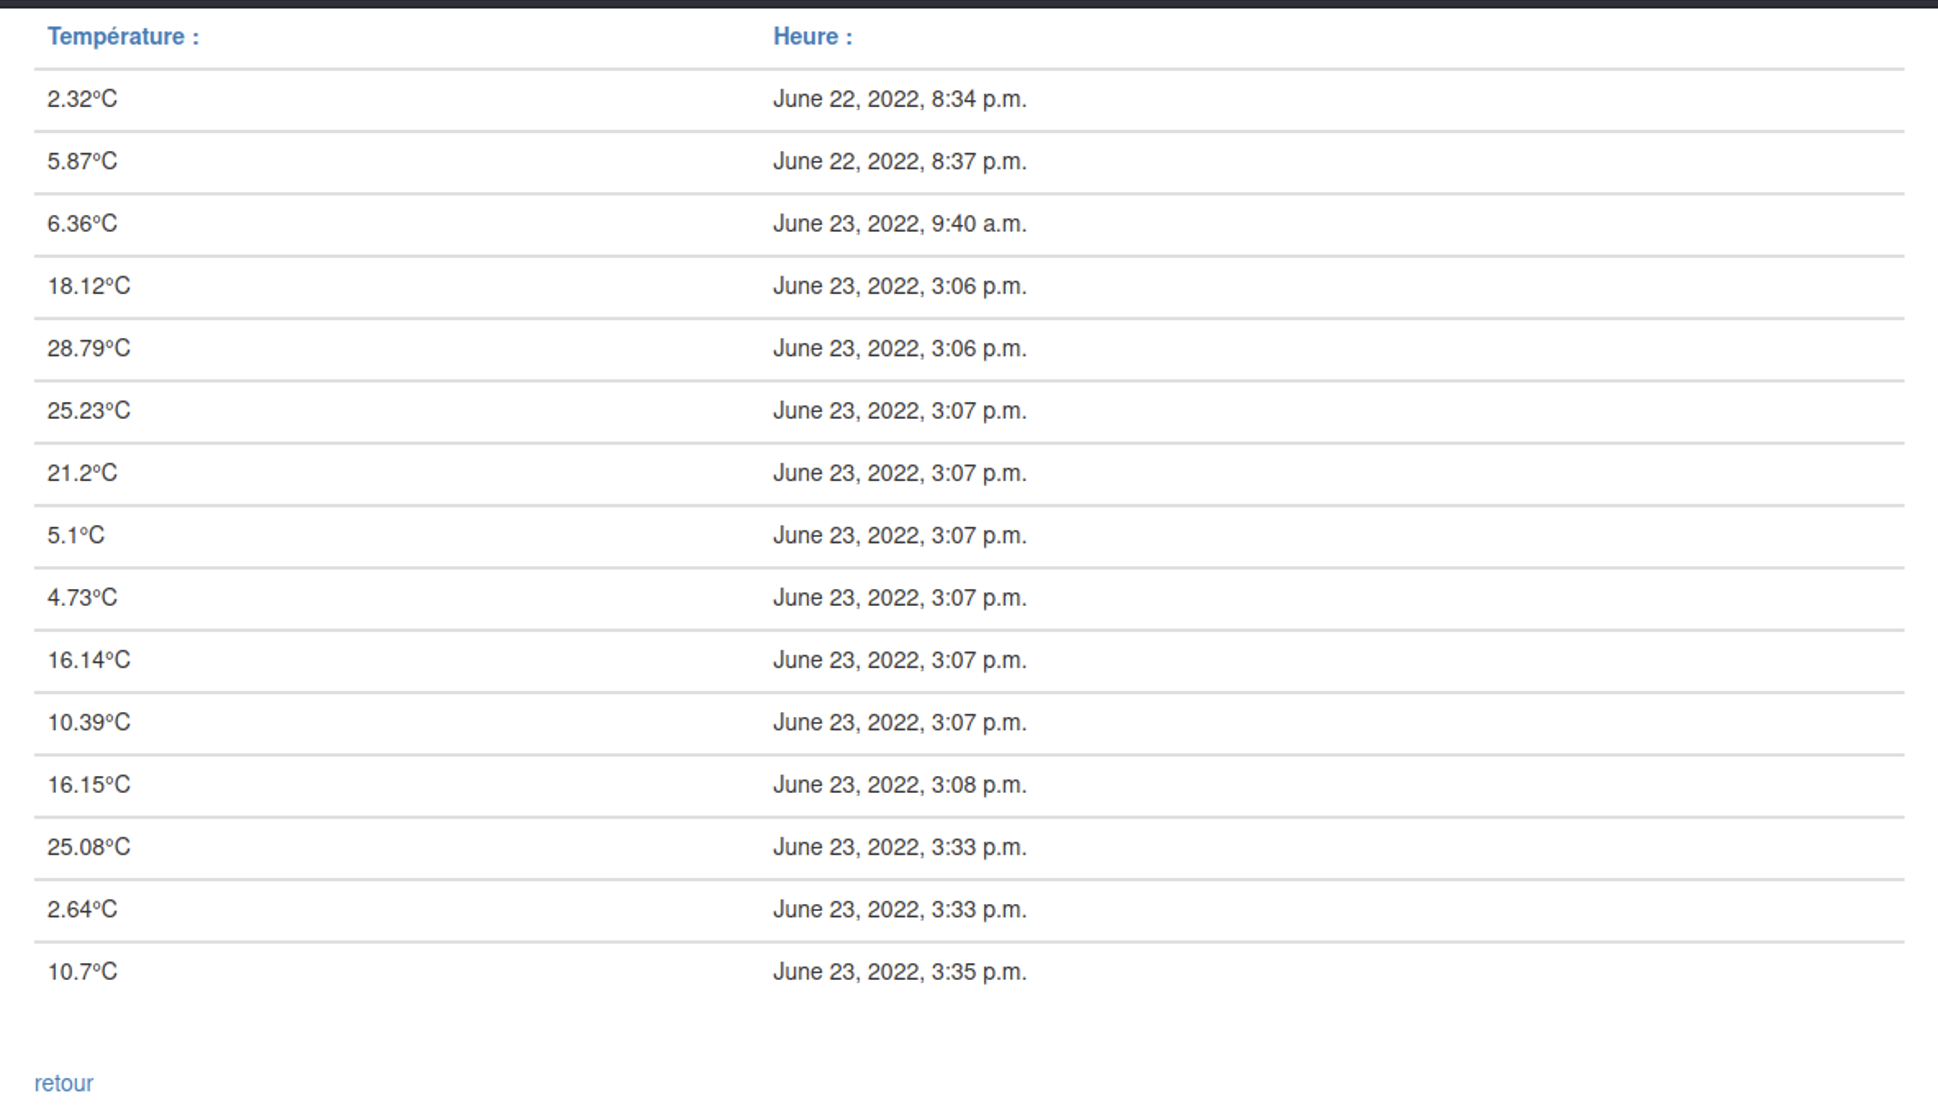
\includegraphics[width=1\textwidth]{../img/data.png}
		\caption{Page de données}
		\label{fig:data}
	\end{figure}
	\newpage 

	\subsection{Mise à jour automatique de la page}

	Pour que nous puissions laisser tourner notre script qui récupère les données, et 
	pouvoir laisser la page des données affiché, nous devons écrire un petit script en javascript
	pour que la page se mette à jour automatiquent. Voici le script que j'ai utilisé :

	\begin{listing}[H]
		\caption{Script pour mettre à jour la page}
		\label{lst:script}
		\begin{minted}{javascript}
		setTimeout(function(){
        		window.location.reload(1);
    		}, 2000);
		\end{minted}
	\end{listing}

	\section{Conclusion}
	En fin de compte, nous avons vu comment créer un projet Django, dépandant d'une base de données, 
	elle-même dépendante d'un script python retransmettant des données transmises en MQTT. 
	Pour finir, cet SAE fût pour nous un gain de connaissances énormes, en réseau, téléphone et 
	programmation. Elle nous a apporté les savoirs qu'il fallait pour pouvoir mener à bien 
	un projet complet et fonctionnel. La compléxité de la tâche ainsi que le temps qui nous était
	accordé (1 jour par partie), nous a appris la gestion du temps et la répartition des tâches. 
	Le fait que nous étions seuls nous a permis d'apprendre à se débrouiller seul, sans 
	forcément dépendre de quelqu'un. 

	







\end{document}